Figure \ref{hardware:block} shows a schematics of the receiver.
Every component is described in more detail in this section.

\begin{figure}[ht]
	\centering
	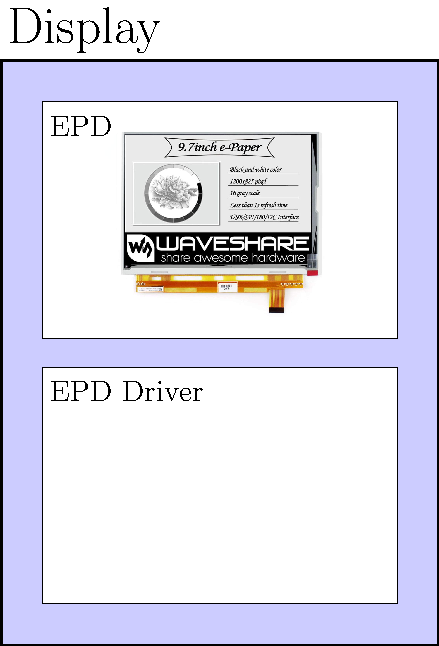
\includegraphics[width=0.9\textwidth]{4-development/hardware/graphics/top/top_schematics.pdf}
	\caption{Receiver schematics.\label{hardware:block}}
\end{figure}

\subsection{Microcontroller}

\subsection{Communication}

\subsubsection{RFicient}

\paragraph{Transmitter}
The Rficient demo kit comes, as previously stated with a \acs{gui}.
Is the transmitter module connected, simple steps make it possible to set the preamble and payload data rate. 
The payload itself can partly serve as an ID and as additional transmitted data.
The power of the transmission can also be set between -30\,dBm and 10\,dBm.
The transmitter-\acs{gui} is shown in Figure \ref{development:tx}.
\begin{figure}[ht]
	\centering
	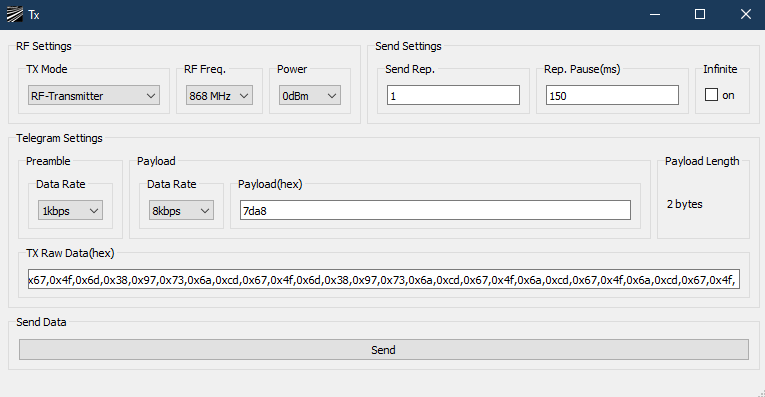
\includegraphics[width=0.9\textwidth]{4-development/hardware/graphics/TXgui.png}
	\caption{Transmitter GUI.\label{development:tx}}
\end{figure}
To test, if any data is received, it is helpful to activate the infinite loop (top right in figure \ref{development:tx}).
The defined data is in this case sent repeatedly with an adjustable period.

\paragraph{Receiver}
To receive the data, the setting of the receiver module need to be matched to the transmitter.
The provided receiver-\acs{gui} makes this step very simple.
As visible in Figure \ref{development:rx}, one can enable the four possible interrupt sources: CodeA/B, ID, FIFO length and FIFO overflow.
In the finished product, it should be possible to wake up the receivers individually.
For this reason, only the ID as interrupt source is of interest.
\begin{figure}[ht]
	\centering
	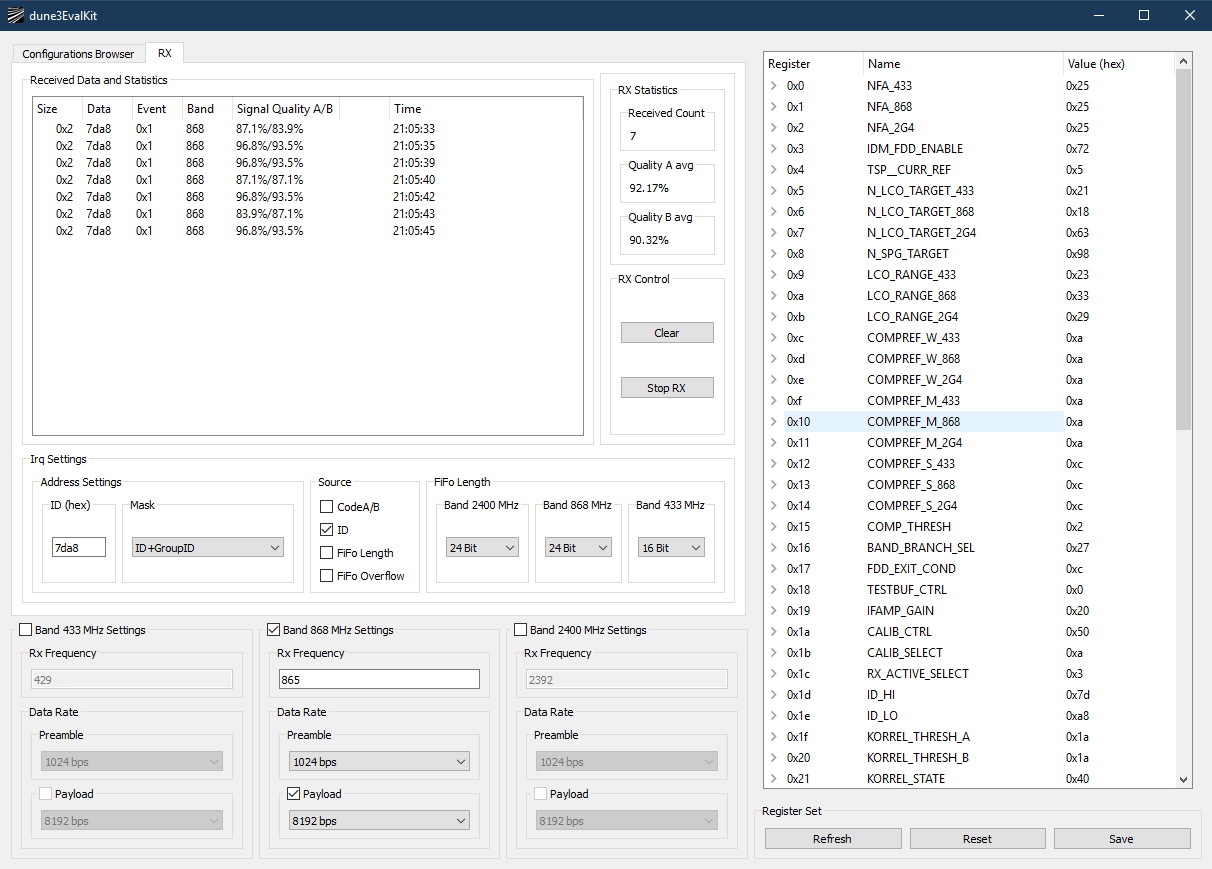
\includegraphics[width=0.9\textwidth]{4-development/hardware/graphics/RXgui.png}
	\caption{Receiver GUI.\label{development:rx}}
\end{figure}
If an interrupt is generated, the RFicient sets a \acs{gpio}-pin to high, and transfers the received data to a \acs{fifo}-buffer.
This data can be passed to a microcontroller over an \acs{spi}-bus.
For the purpose of this thesis, only the \acs{gpio} high level is used as a on switch of a self-holding circuit.

\paragraph{Tests in a realistic environment}
To test the RFicient in more detail, some indoor measurements were made.
As test environment served several buildings of the \acf{hsr}, since this type of facility represents a realistic condition for the developed schedule.

Purpose of the first test was to measure the achievable range.
Figure \ref{development:env1} shows the hallway where this test was executed.
\begin{figure}[ht]
	\centering
	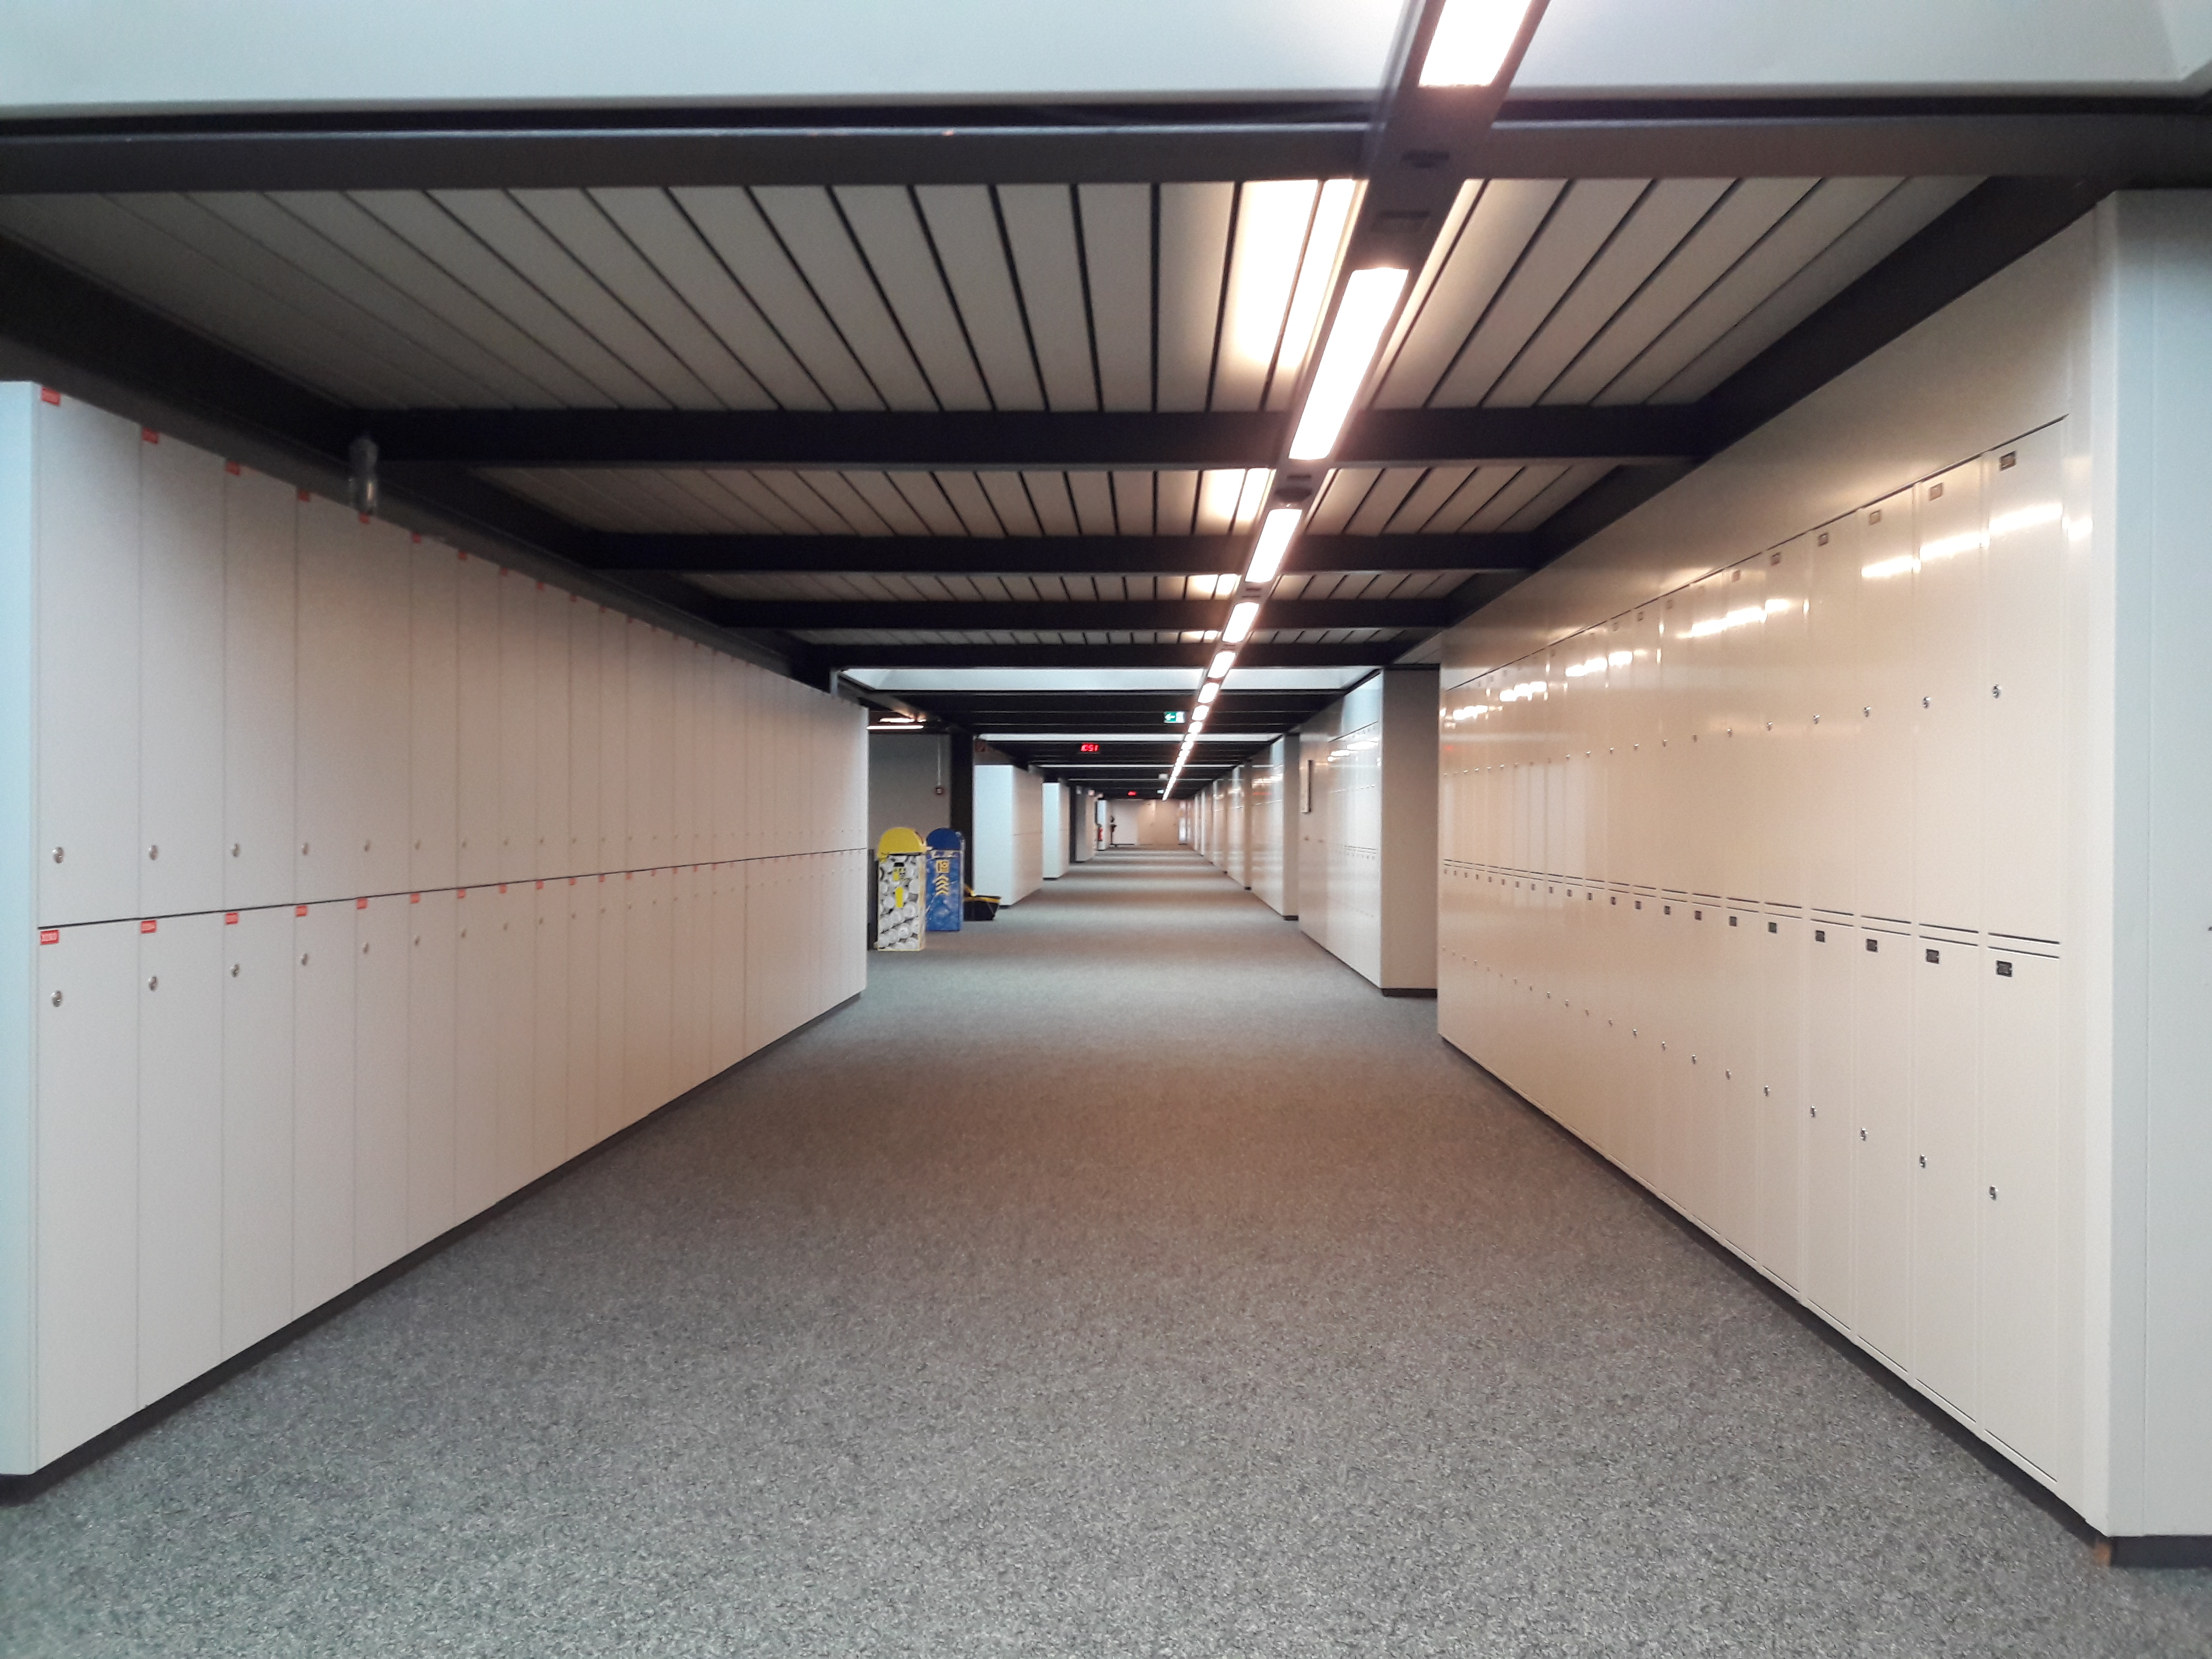
\includegraphics[width=0.9\textwidth]{4-development/hardware/graphics/env1.jpg}
	\caption{Test environment 1 (\acs{hsr} building 1).\label{development:env1}}
\end{figure}
With a transmission power of 0\,dBm (1\,mW) it is possible to receive interrupt over a 50\,m distance (line of sight).
Is the transmission power increased to 10\,dBm (10\,mW), interrupts can be sent over a distance up to 80\,m.
In this environment, the Rficient has enough range.
But maybe reflections off the walls, floor and ceiling have contributed to this result.

Out if this reason, a second test was performed to check how the RFicient penetrates obstacles.
As test environment served this time the \acs{hsr} builing 8, as depicted in Figure \ref{development:env2}.
An attempt was made to send wakeup signals through the ceiling.
\begin{figure}[ht]
	\centering
	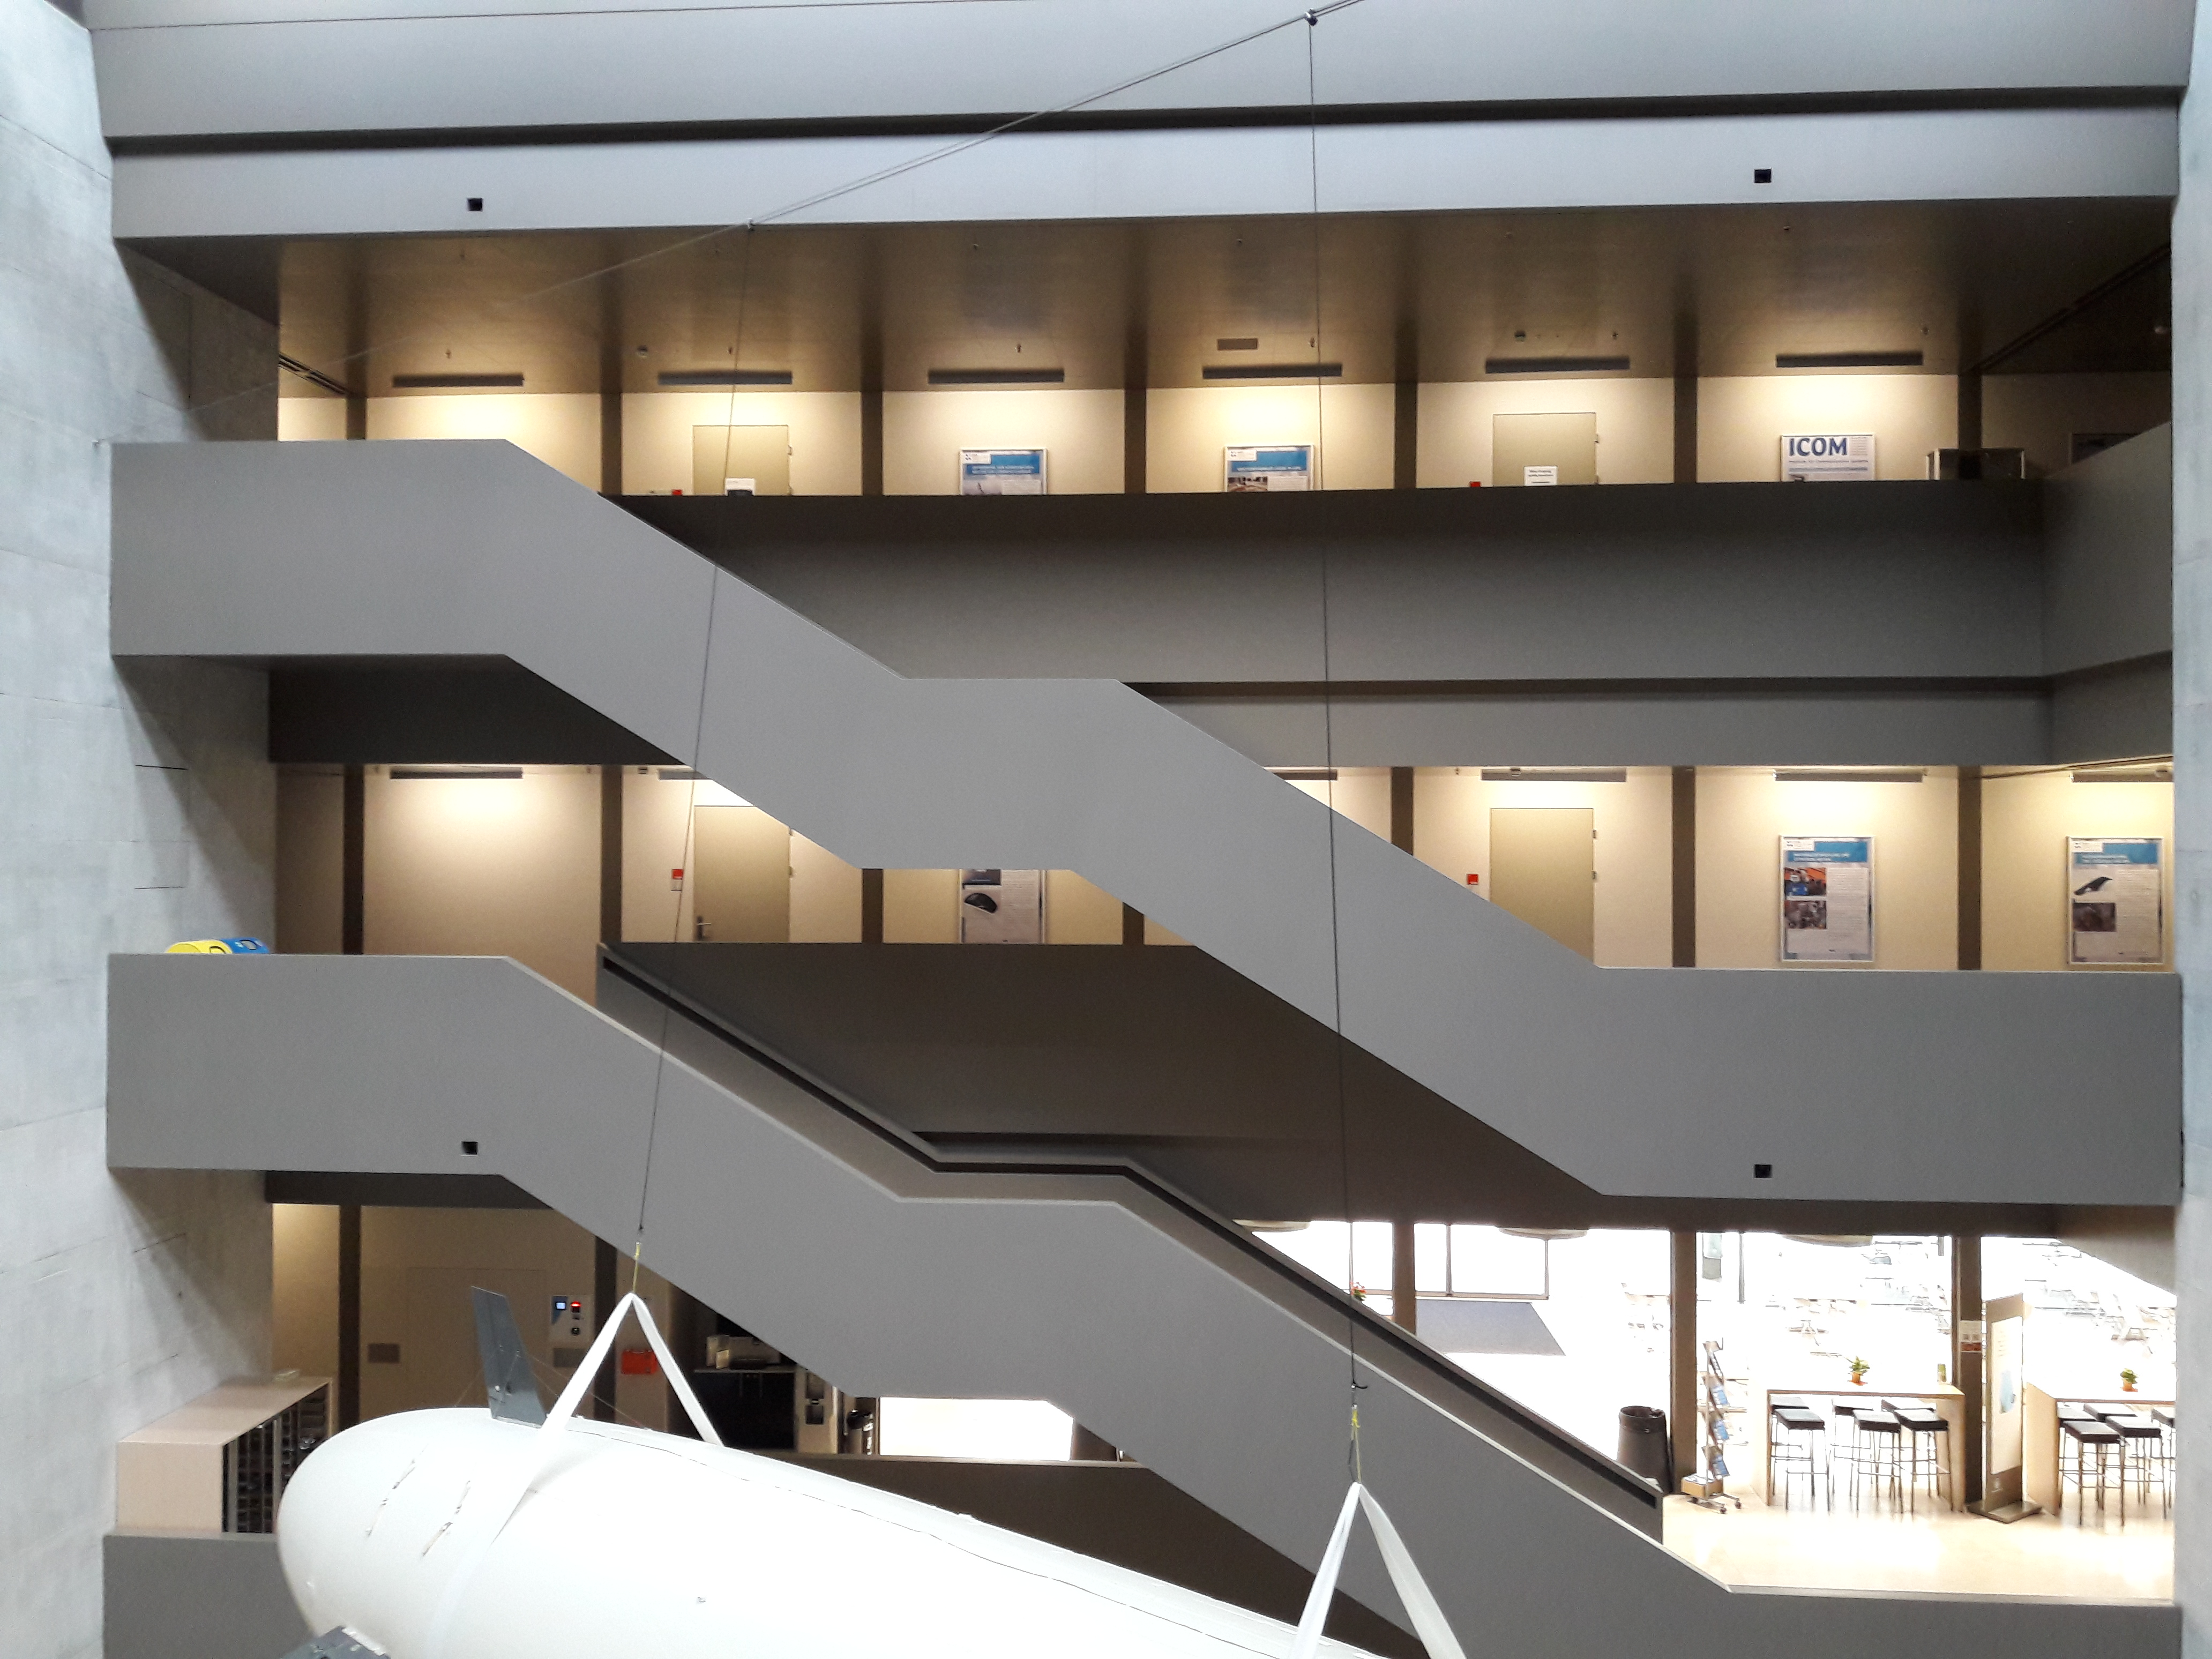
\includegraphics[width=0.9\textwidth]{4-development/hardware/graphics/env2.jpg}
	\caption{Test environment 2 (\acs{hsr} building 8).\label{development:env2}}
\end{figure}
To avoid reflections, the RFicient was placed in such a way, that the zero point of the antenna pointed directly at the opposite walls.
With a transmisson power of 0\,dBm, two ceilings can be penetrated.
Is the power again increased to 10\,dBm, the signal reached through three ceilings.

These measurements further confirmed, that the RFicient is suitable for the use-case of this semester thesis.

\subsubsection{nRF52480}
A nRF52580 from nordic semiconductor serves as the wireless module.
It is used because it supports multiple protocols like Thread, Zigbee and more important Bluetooth 5 which includes \acf{ble}\cite{nrfpb}.
Since \acs{ble} allows mesh networking and is applied in many existing devices, such as smartphones, the connection to transmit data is established over this protocol.
This way, the developed prototype could later be extended to a mesh network.

Two nRF52480 development kits are used, one on transmitter and one on receiver end.
Data can be transferred from a computer with a \acs{usb}-\acs{ttl}-adapter to the \acs{uart}-interface of the transmitter development kit.
This data is then sent over \acs{ble} to the receiver kit and passed to the microcontroller again over \acs{uart}.
In the same way, data can be transferred from the receiver to the transmitter kit.
The data channel is therefore bi-directional. 

\subsection{Power Management}
The screen should be self-sustaining, thus some sort of energy-harvesting unit is needed.
It was apparent to choose light as the energy source, since the screen will be used in rooms, that are artificially illuminated most of the time.
The energy  obtained by solar cells is converted to a suitable voltage, using a ADP5090 chip.
This way, a super-capacitor, which is used as an energy storage device, is charged.

\subsubsection{Solar cell}
As solar cell, the AM-1522 by Panasonic is used.
One panel has an area of $55.0\,\text{mm}\,\times\,40.5\,\text{mm}$ and delivers up to $58.7\, \mu\text{A}$ when operating at an optimal voltage of $2.1\,\text{V}$, provided an illuminance of 200\,lux.
To keep a reasonable display to panel ratio, four cells where connected in parallel, which corresponds to an area of ca. $89.1\,\text{cm}^2$ (Display area = $283\,\text{cm}^2$). Therefore, the solar cells should provide a power of

\begin{align}
	P = U\cdot I = 4\cdot 57.8\,\mu\text{A}\cdot 2.1\ \text{V}=485.52\,\mu \text{W},\label{development:cell_power}
\end{align}

given a 200 lux illuminance \cite{amorton}.

\subsubsection{ADP5090}
The ADP5090 from Analog Devices is used to manage the energy harvesting process.
This boost regulator makes it possible to charge storage elements, such as rechargeable batteries and super capacitors with the input dc-power provided by the PV-cell. Utilized features are:
\begin{itemize}
	\item[-] Maximum power point tracking
	\item[-] Efficiency up to 90\%
	\item[-] Input voltage $V_{IN}$ from $80\,\text{mV}$ to $3.3\,\text{V}$
	\item[-] Programmable voltage range ($2.2\,\text{V}$ to $5.2\,\text{V}$) for the storage element
\end{itemize}
To prevent the storage element from overdischarging, the ADP5090 enables the user to set a maximal Voltage with resistors:

\begin{align}
	V_{\text{BAT\_TERM}} = \frac{3}{2} V_{\text{REF}}\left(1+\frac{R_{\text{TERM1}}}{R_{\text{TERM2}}} \right).\label{development:v_bat_term} 
\end{align} 

The same procedure is applied to set a minimal voltage:

\begin{align}
	V_{\text{BAT\_SD}}=V_{\text{REF}} \left(1+\frac{R_{\text{SD1}}}{R_{\text{SD2}}} \right).\label{development:v_bat_sd} 
\end{align}  

While discharging, the ADP5090 will switch off the output $V_{\text{SYS}}$ if $V_{\text{BAT\_SD}}$ is reached. This prevents the storage element from overdischarging.
The output voltage $V_{\text{SYS}}$, where the load is attached, will therefore always stay in this programmed range $(V_{\text{BAT\_SD}}\le V_{\text{SYS}}\le V_{\text{BAT\_TERM}})$ \cite{adp}.

For this prototype, the evaluation board for the ADP5090 was used, where the internal reference voltage ($V_{\text{REF}}$ in \eqref{development:v_bat_term} and \eqref{development:v_bat_sd}) is $1.21\,\text{V}$ \cite{adp_eval}.

\subsubsection{Super capacitor}
As energy storage, a super capacitor from Taiyo Yuden (LIC1235RS3R8406) has proven to be suitable, which is a $40\,\text{F}$ cylinder type lithium ion capacitor.
The operating voltage range is between $2.2\,\text{V}$ and $3.8\,\text{V}$.
Discharging the capacitor lower than $2.2\,\text{V}$ causes shorter lifetime and higher leakage current.
The same unwanted behaviour occurs when charging the capacitor over $3.8\,\text{V}$ \cites{yuden}.

\subsubsection{Combined test}
To test the behaviour of the power management, supercapacitor and solar cells, a couple of measurements are executed.
Figure \ref{development:test} shows the layout of the test setup.

\begin{figure}[ht]
	\centering
	
\includegraphics[width=0.9\textwidth]{4-development/hardware/graphics/testaufbau.pdf}
	\caption{Schematics of the test setup.\label{development:test}}
\end{figure}

To carry out these measurements, it is first necessary to adjust the minimal and maximal voltage of the ADP5090.
The nrf58240 accepts supply voltages between $1.6\,\text{V}$ up to $5.5\,\text{V}$ \cite{nrf}.
The STM32 on the other side is less flexible with an input voltage range of $1.71\,\text{V}$ to $3.6\,\text{V}$ \cite{stm32}.
As stated in the section above, the super capacitors operating voltage is between $2.2\,\text{V}$ and $3.8\,\text{V}$.
Hence it seems reasonable, to set $V_{\text{BAT\_TERM}} \le 3.6\,\text{V}$ and $V_{\text{BAT\_SD}} \ge 2.2\,\text{V}$, to satisfy all of these three elements.
In order to do this, the four resistors have to be chosen as $R_3 = 4.3\,\text{M}\Omega$, $R_6 = 4.7\,\text{M}\Omega$, $R_2 = 4.3\,\text{M}\Omega$ and $R_3 = 5.1\,\text{M}\Omega$.
Inserted in the equation \eqref{development:v_bat_term} and \eqref{development:v_bat_sd} we get
\begin{align}
	V_{\text{BAT\_TERM}}= \frac{3}{2} 1.21\,\text{V} \left(1 + \frac{4.3\,\text{M}\Omega}{4.7 \,\text{M}\Omega} \right) \approx 3.48\,\text{V} 
\end{align}
and
\begin{align}
	V_{\text{BAT\_SD}} = 1.21\,\text{V} \left(1 + \frac{4.3\,\text{M}\Omega}{5.1\,\text{M}\Omega} \right) \approx 2.23\,\text{V}. 
\end{align}

While testing, the input voltage from the solar cells ($V_{\text{IN}}$), voltage of the supercap ($V_{\text{BAT}}$) and the output voltage ($V_{\text{SYS}}$) are tracked. Additionally, the illuminance ($E_\text{v}$) near the PV-cells  is recorded as indicated in figure \ref{development:test}.

The purpose of the first test is to check, if the ADP5090 converts $V_{\text{IN}}$ to a voltage $\le V_{\text{BAT\_TERM}}$.
The measurements where taken over a couple hours and are plotted in Figure \ref{development:charge}.

\begin{figure}[ht]
	\centering
	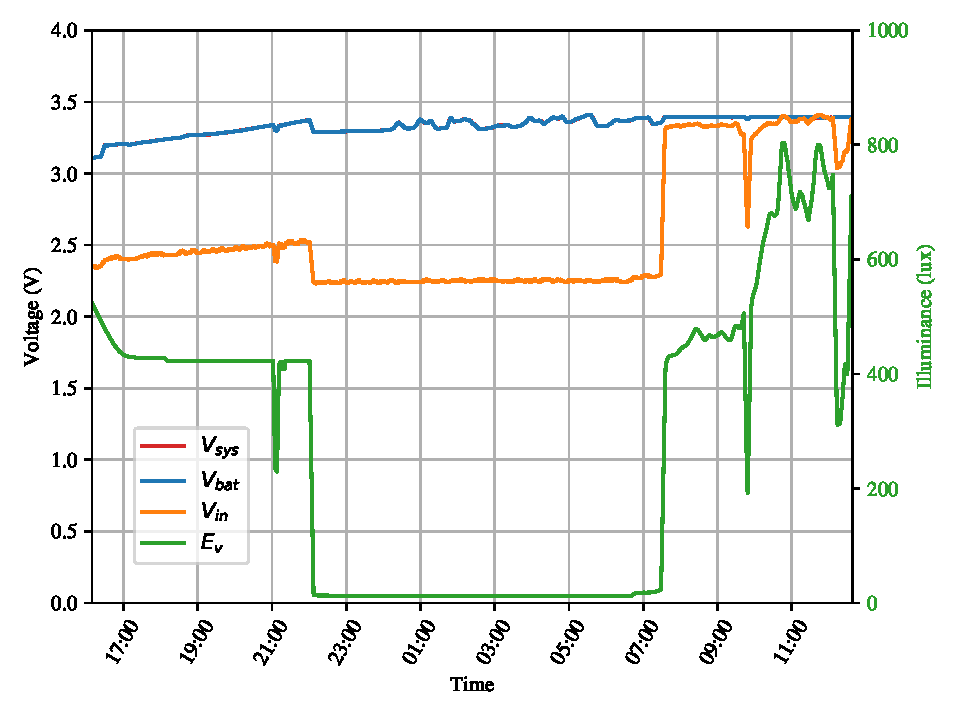
\includegraphics[width=0.9\textwidth]{4-development/hardware/graphics/laden.pdf}
	\caption{Charging behaviour.\label{development:charge}}
\end{figure}

No load was connected to the output ($Z_\text{LOAD} \to \infty$), which is the reason $V_{\text{SYS}}$ is overlapped by $V_{\text{BAT}}$.
It can be seen, that between 17:00 and 23:00, the super capacitor was being charged and
that the ADP5090 controls the voltage $V_{\text{BAT}}$ like expected to the adjusted maximum voltage $V_{\text{BAT\_TERM}}$.

The second test should simulate the discharging when a load is connected, after the capacitor was fully charged.
It was necessary to estimate the consumed power by the electronic components of the prototype.
A rough measurement with a power analyser showed, that the microcontroller and the e-paper display together draw at its peak about $240\,\text{mA}$ when connected to $5\,\text{V}$. The nrf52840 on the other hand, only consumes 6 mA with a 3 V source. Thus the expected consumed power at is's peak is:
\begin{align}
	P_{e} = 5\,\text{V}\cdot 0.24\,\text{A} + 3\,\text{V}\cdot 0.006\,\text{A} = 1.218\,\text{W}.
\end{align}
  

If $Z_{\text{LOAD}}=10\,\Omega$ the load draws currents between $0.223\,\text{A}$ and $0.348\,\text{A}$ which again lead to a power consumption that should approximately match the power consumption of the finished prototype.
Furthermore, the solar cells where covered to observe the discharging without interference of additionally charging behaviour.
Figure \ref{development:discharge} shows the result.
 
\begin{figure}[ht]
	\centering
	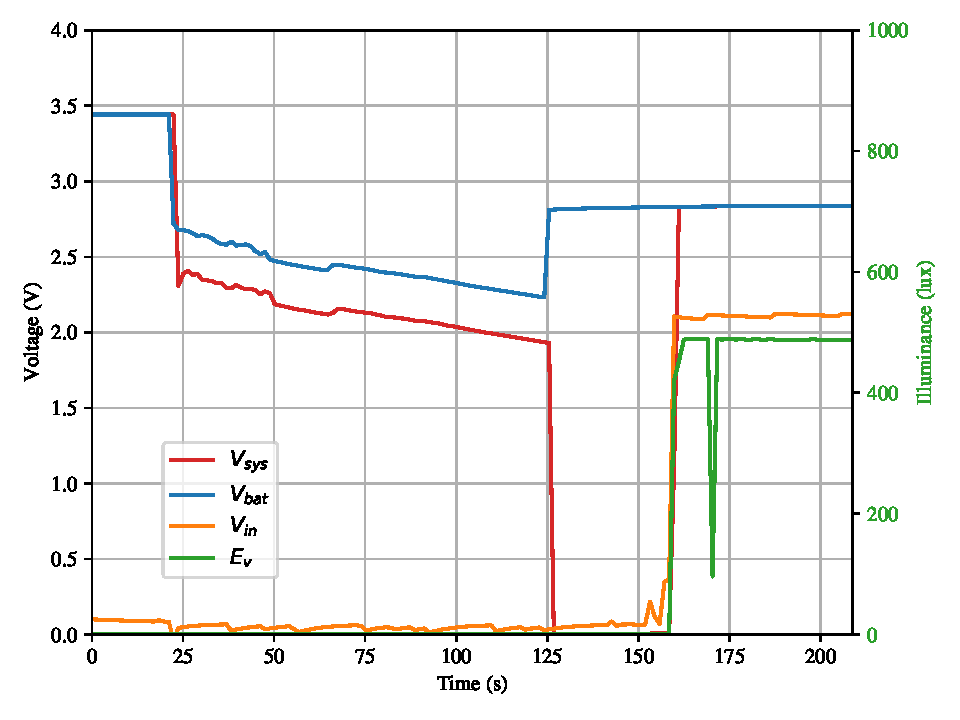
\includegraphics[width=0.9\textwidth]{4-development/hardware/graphics/entladen.pdf}
	\caption{Discharging behaviour.\label{development:discharge}}
\end{figure}

As soon as the load is connected (after 25\,), $V_{\text{SYS}}$ and $V_{\text{BAT}}$ first drop by almost $1\,\text{V}$ and after that steadily decrease.
After ca. 100 s, $V_{\text{BAT}}$ reached the value of $V_{\text{BAT\_SD}}$ and the ADP5090 switches the output off ($V_{\text{SYS}}$ drops to 0) to prevent the capacitor from overdischarging.
The output now stays switched off, until $V_{\text{IN}}$ again supplies energy, and $V_{\text{BAT}} \le V_{\text{BAT\_SD}}$.
It can also clearly be seen, that after 160 seconds, the ADP5090 controls $V_{\text{IN}}$ to ca. $2.1\,\text{V}$. Recall that this is the optimal power point of the solar cell.

\subsection{Display}
